\begin{frame}[fragile]{Thesis Goal} % some commands, e.g. \verb require [fragile]
\begin{itemize}
  \item Learning System Models\\%\pause, <-- put these in here later
  \item Navigation Among Movable Objects\\
  \item Nonprehensile Pushing
\end{itemize}
\end{frame}

\begin{frame}[fragile]{Robot Environment} % some commands, e.g. \verb require [fragile]
\begin{center}
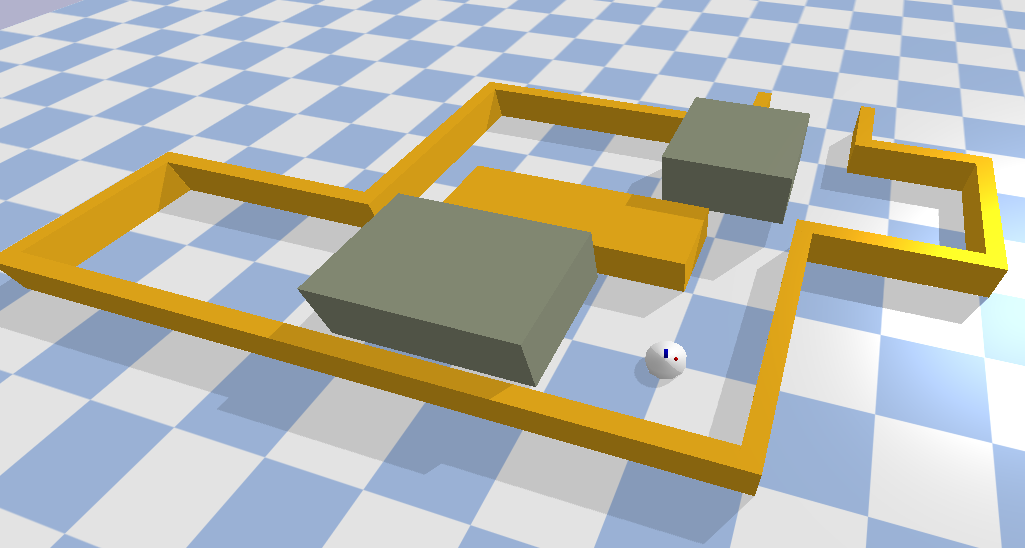
\includegraphics[width=0.7\textwidth]{figures/introduction/2_pushes_to_freedom}
\end{center}
\end{frame}


\begin{frame}[fragile]{Joint Configuration Space}
\begin{center}
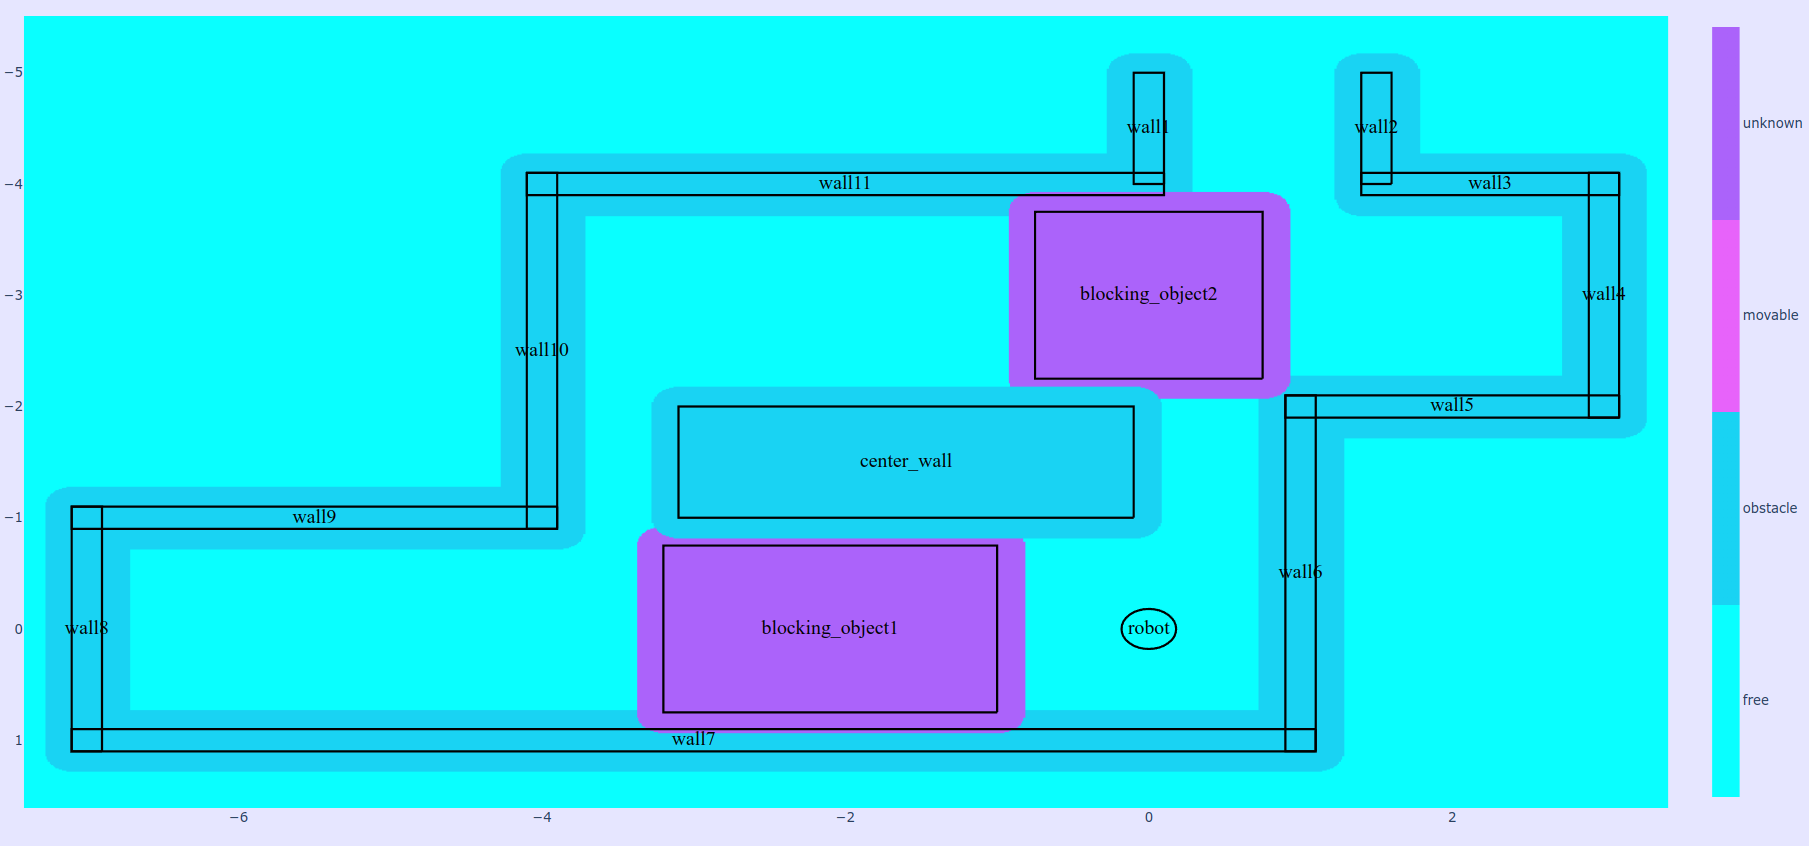
\includegraphics[width=0.6\textwidth]{figures/introduction/2_pushes_to_freedom_robot_conf_space}\vspace{2mm}
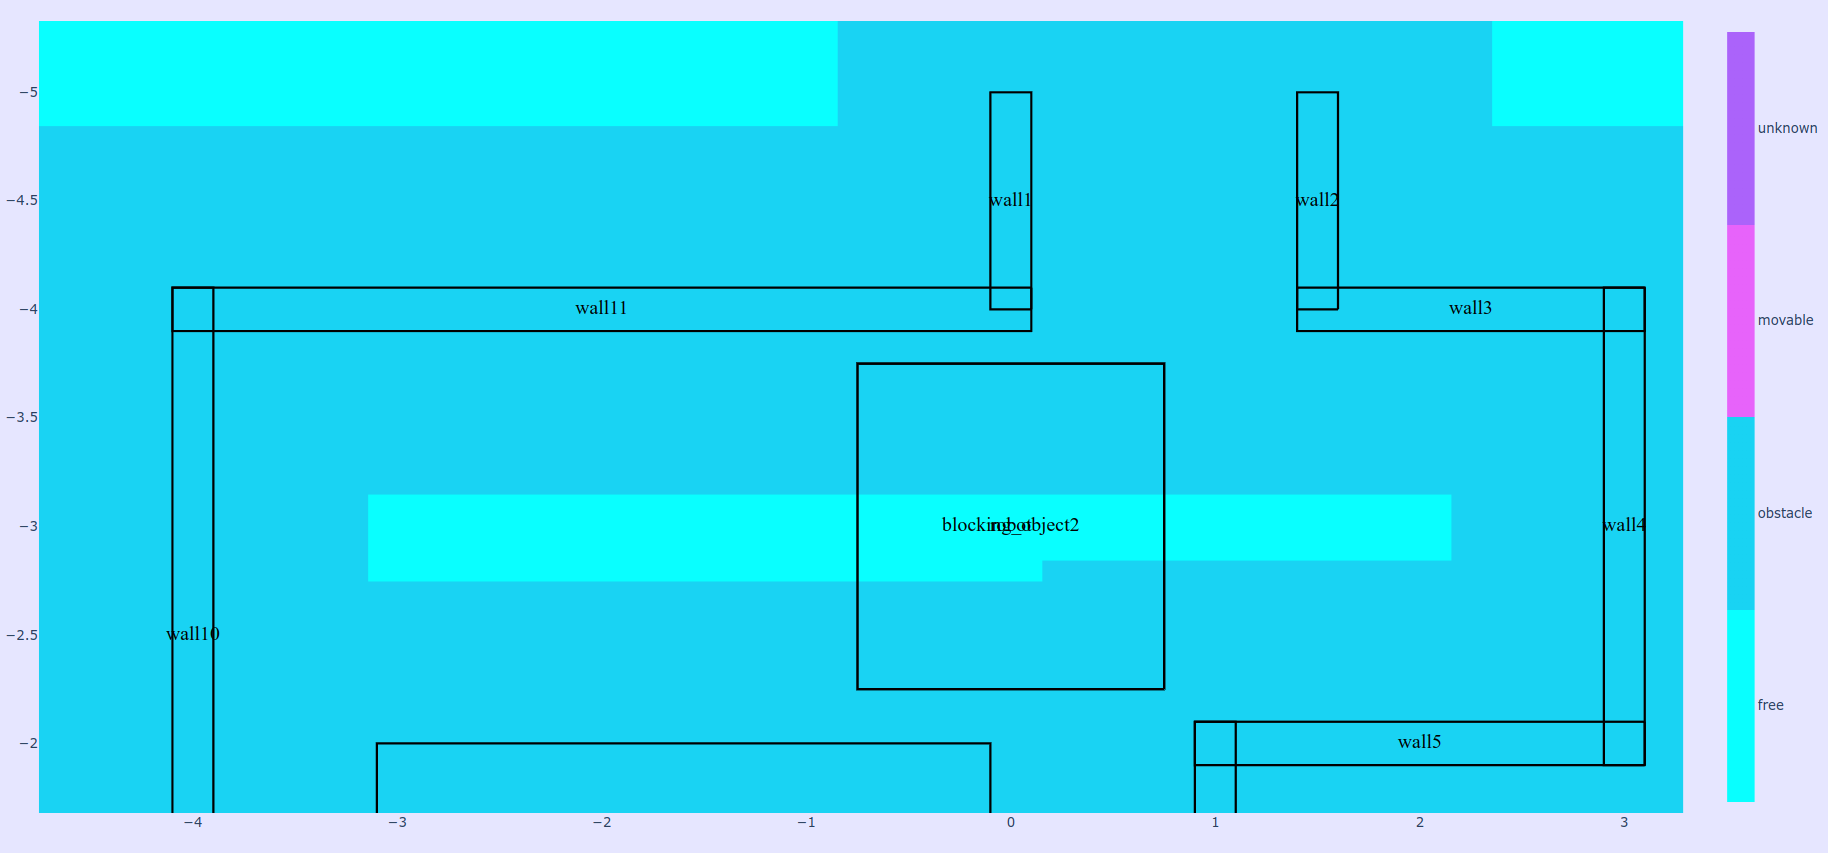
\includegraphics[width=0.6\textwidth]{figures/introduction/2_pushes_to_freedom_box_conf_space}
\end{center}
\end{frame}


\begin{frame}[fragile]{Research Question}
\large
How do learned objects' system models improve global task planning for a robot with nonprehensile push manipulation abilities over time?\bs

\textbf{Research Subquestions:}
\begin{enumerate}
  \item Can the proposed method combine learning and planning for push en drive applications with a technique known as backward search?\\
  \item How do learning system models and remembering interactions compare to only learning system models? And, how does the proposed method compare against the state-of-the-art?
\end{enumerate}
\end{frame}

\begin{frame}[fragile]{State-of-The-Art}
\begin{table}[H]
  \centering
  \begin{tabular}
  {>{\raggedright\arraybackslash}p{2.0cm}%
    ccc%
    >{\raggedright\arraybackslash}p{2.5cm}}
    Author &  Learning & NAMO & Object to Target & Manipulation\\[2mm]
    \citeauthor{ellis_navigation_2022}  &\cmark& \cmark& \xmark& pushing\\
    \citeauthor{sabbaghnovin_model_2021} & \cmark& \xmark& \cmark& grasp-push grasp-pull\\
    \citeauthor{scholz_navigation_2016} & \cmark& \cmark& \xmark& graph-push grasp-pull\\
    \citeauthor{vega-brown_asymptotically_2020} & \xmark& \cmark& \cmark& gripping\\[2mm]
    \citeauthor{wang_affordancebased_2020} & \cmark& \cmark& \xmark& pushing\\
    Groote & ? & ? & ? & pushing\\
  \end{tabular}
\end{table}
\end{frame}

\begin{frame}[fragile]{Robot Environment}
  \todo{make slide}

\end{frame}

\begin{frame}[fragile]{Assumptions}
  \todo{make slide}

\end{frame}


\begin{frame}[fragile]{Task Specification}
  \todo{make  slide}

\end{frame}
